%% effector_characteristics.tex
%% Copyright: James Hutton Institute 2016
%% Author: Leighton Pritchard
%% Effector characteristics

% WHAT IS AN EFFECTOR (MAP)
\begin{frame}
  \frametitle{What is an effector?}
  \begin{center}
    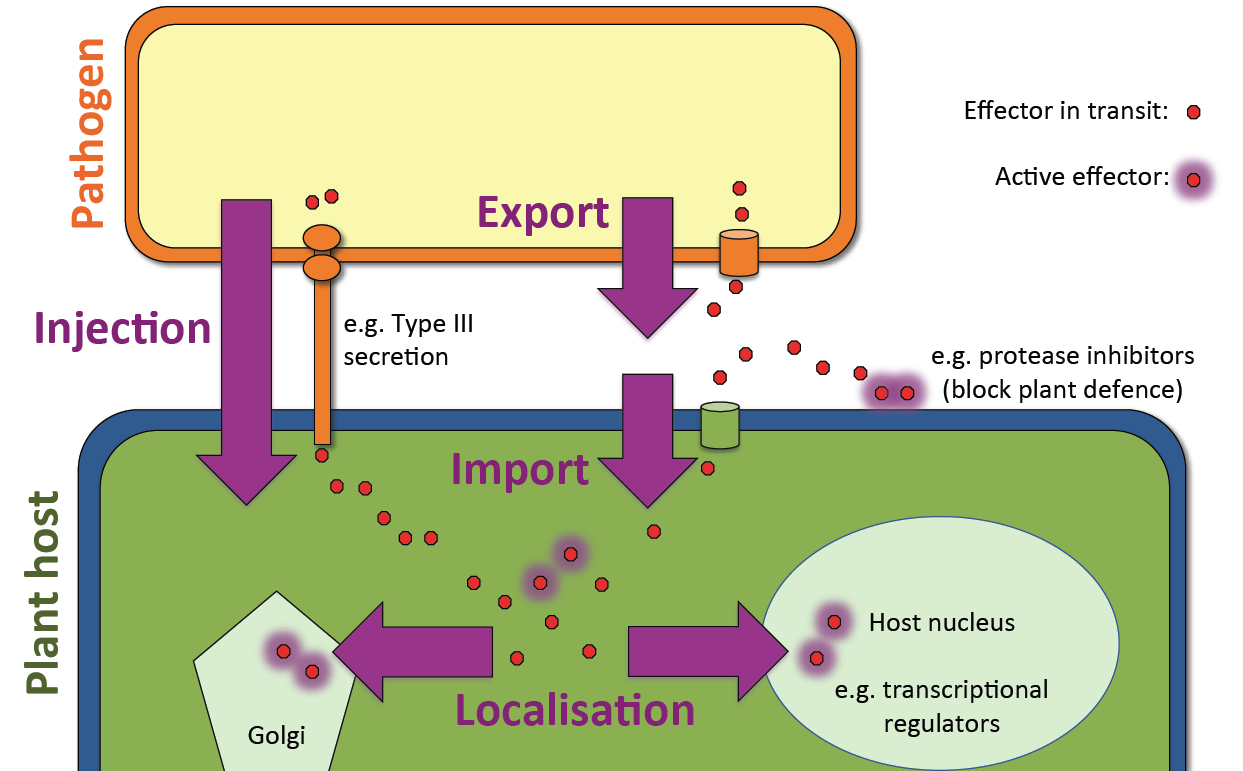
\includegraphics[width=1\textwidth]{images/effector_map}    
  \end{center}
\end{frame}

% WHAT IS AN EFFECTOR (DEFINITION)
\begin{frame}
  \frametitle{What is an effector?}
  \begin{alertblock}{Effector}
    A molecule produced by pathogen that (directly?) modifies host molecular/biochemical `behaviour'
  \end{alertblock}
  \begin{itemize}
    \item \textcolor{hutton_blue}{Inhibits enzyme action} 
    {\footnotesize (e.g. \textit{Cladosporium fulvum} AVR2, AVR4; \textit{Phytophthora infestans} EPIC1, EPIC2B; \textit{P. sojae} glucanase inhibitors)}
    \item Cleaves a protein target  
      {\footnotesize (e.g. \textit{Pseudomonas syringae} AvrRpt2)}
    \item \textcolor{hutton_green}{(De-)phosphorylates a protein target}  
      {\footnotesize (e.g. \textit{P. syringae} AvrRPM1, AvrB)}
    \item Retargeting host system such as E3 ligase  
      {\footnotesize (e.g. \textit{P. syringae} AvrPtoB; \textit{P. infestans} Avr3a)}
    \item \textcolor{hutton_purple}{Regulatory control}  
      {\footnotesize (e.g. \textit{Xanthomonas campestris} AvrBs3)}
  \end{itemize}
\end{frame}

% WHAT IS AN EFFECTOR (ELEPHANT)
\begin{frame}
  \frametitle{What is an effector?}
  No unifying biochemical mechanism \\
  \textcolor{red}{No single test for `candidate effectors'}, even in one organism
  \begin{center}
    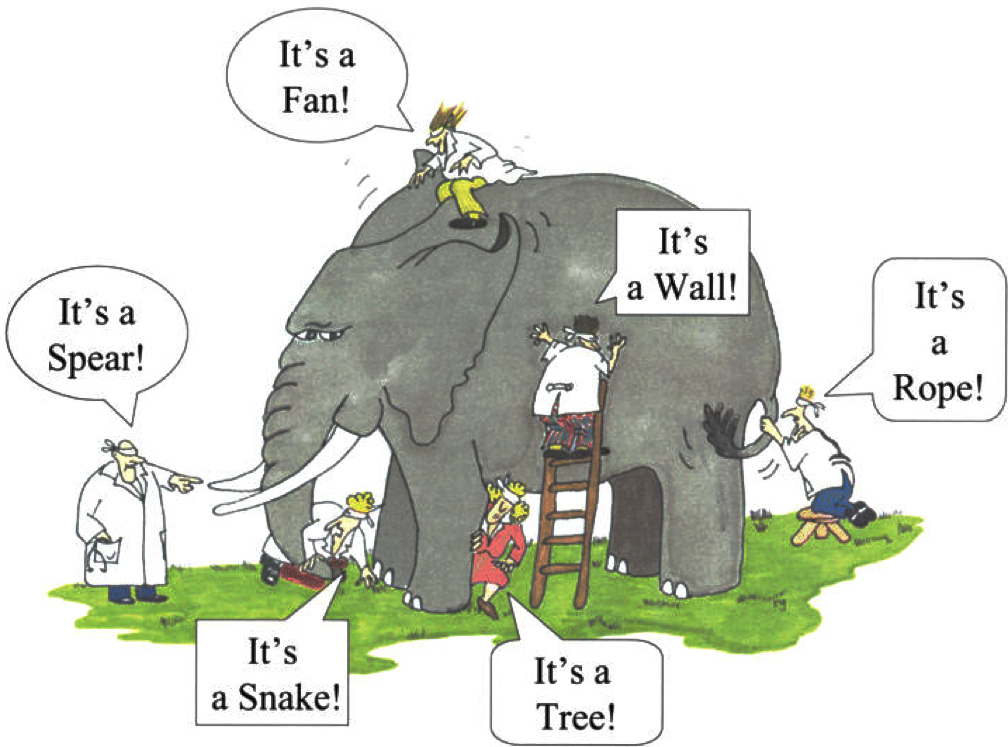
\includegraphics[width=0.8\textwidth]{images/elephant}    
  \end{center}
\end{frame}


% EFFECTORS ARE MODULAR 1
\begin{frame}
  \frametitle{Effectors are modular
  \footnote{\tiny{\href{http://dx.doi.org/10.1016/S1369-5274(02)00004-8}{Greenberg \& Vinatzer (2003) \textit{Curr. Opin. Microbiol.} doi:10.1016/S1369-5274(02)00004-8}}}
  \footnote{\tiny{\href{http://dx.doi.org/10.1016/S0966-842X(02)02451-4}{Collmer \textit{et al.} (2002) \textit{Trends Microbiol.} doi:10.1016/S0966-842X(02)02451-4}}}
  }
  \begin{footnotesize}
    \begin{alertblock}{Delivery}
      N-terminal localisation/translocation domain
    \end{alertblock}
    \begin{block}{Activity}
      C-terminal functional/interaction domain
    \end{block}  
  \end{footnotesize}
  \begin{center}
    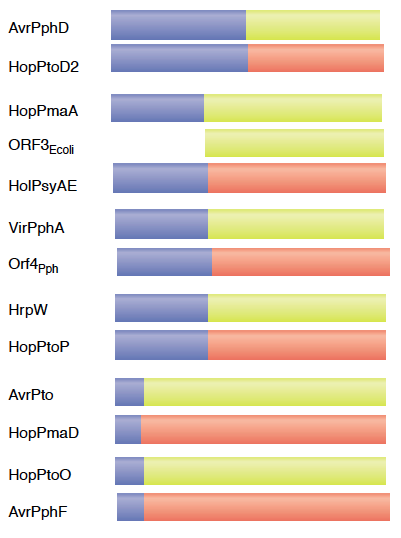
\includegraphics[height=0.425\textheight]{images/modular_t3ss_greenberg_2003}    
    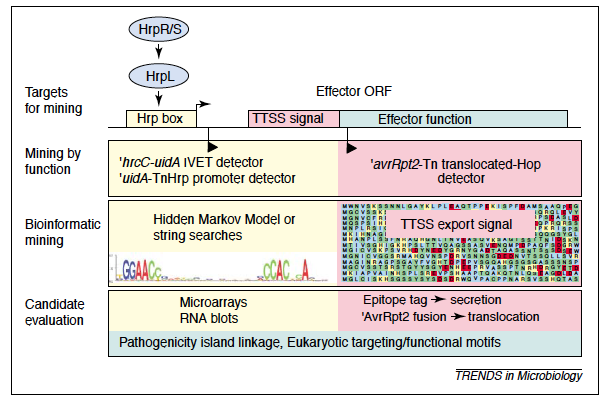
\includegraphics[height=0.425\textheight]{images/modular_ttss_collmer_2002}        
  \end{center}
\end{frame}

% EFFECTORS ARE MODULAR 2
\begin{frame}
  \frametitle{Effectors are modular
  \footnote{\tiny{\href{http://dx.doi.org/10.1371/journal.pone.0020172.t004}{Dong \textit{et al.} (2011) \textit{PLoS One} doi:10.1371/journal.pone.0020172.t004}}}
  \footnote{\tiny{\href{http://dx.doi.org/10.1126/science.1178811}{Boch \textit{et al.} (2009) \textit{Science} doi:10.1126/science.1178811}}}
  }
  \begin{footnotesize}
    \begin{alertblock}{Delivery}
      Typically common to effector class: RxLR, T3E, CHxC
    \end{alertblock}
    \begin{block}{Activity}
      May be common (TAL) or divergent within effector class (RxLR, T3E)
    \end{block}  
  \end{footnotesize}
  \begin{center}
    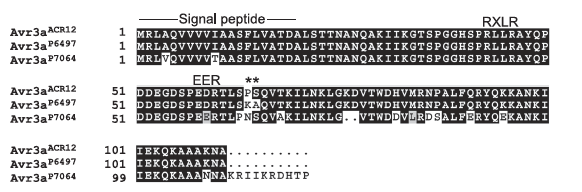
\includegraphics[width=0.6\textwidth,valign=t]{images/modular_rxlr_dong_et_al_2011}    
    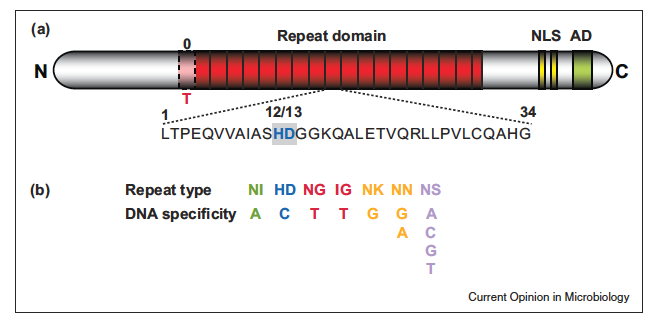
\includegraphics[width=0.4\textwidth,valign=t]{images/modular_tal_scholze_et_al_2011}        
  \end{center}
\end{frame}

% EFFECTOR PREDICTORS
\begin{frame}
  \frametitle{Effector prediction tools (online)
  \footnote{\tiny{\href{http://dx.doi.org/10.1371/journal.ppat.1004806}{Sperschneider \textit{et al.} (2015) \textit{PLoS Pathogens} doi:10.1371/journal.ppat.1004806}}}
  \footnote{\tiny{\href{http://dx.doi.org/10.3389/fpls.2016.00126}{Sonah \textit{et al.} (2016) \textit{Front. Plant Sci.} doi:10.3389/fpls.2016.00126}}}
  }
  \begin{alertblock}{Bacterial Type III Effectors}
    \begin{itemize}
      \item \textcolor{hutton_purple}{\href{http://www.effectors.org/method/effectivet3}{EffectiveT3}}
      \item \textcolor{hutton_purple}{\href{http://gecco.org.chemie.uni-frankfurt.de/T3SS_prediction/T3SS_prediction.html}{modlab}}
      \item \textcolor{hutton_purple}{\href{http://effectors.bic.nus.edu.sg/T3SEdb/predict.php}{T3SEdb}}
    \end{itemize}
  \end{alertblock}
  \begin{block}{Fungal/Oomycete Effectors}
    \begin{itemize}
      \item \textcolor{hutton_purple}{\href{http://effectorp.csiro.au/}{EffectorP}}
      \item \textcolor{hutton_purple}{\href{http://bit.ly/1XHf0kM}{Galaxy Toolshed RxLR predictor}}
    \end{itemize}
  \end{block}
\end{frame}


% WHAT DO WE LOOK FOR
\begin{frame}
  \frametitle{What do we look for?
  \footnote{\tiny{\href{http://dx.doi.org/10.1007/978-1-62703-986-4_4}{Pritchard \& Broadhurst (2014) \textit{Methods Mol. Biol.} doi:10.1007/978-1-62703-986-4\_4}}}
  }
  What if someone hasn't built a classifier for your protein family?
      \begin{itemize}  
        \item \textcolor{hutton_green}{Tests are for protein family membership and/or `effector-like' functional signal}
        \item \textcolor{hutton_blue}{The same as any sequence classification problem (functional annotation)}
        \item \textcolor{hutton_purple}{Many possible approaches}
        \item \textcolor{RawSienna}{(Supervised) machine learning problem:}
        \begin{itemize}
          \item train
          \item test
          \item validate
        \end{itemize}
      \end{itemize}
\end{frame}

% SEQUENCE SPACE
\begin{frame}
  \frametitle{Sequence space
  \footnote{\tiny{\href{http://dx.doi.org/10.1007/978-1-62703-986-4_4}{Pritchard \& Broadhurst (2014) \textit{Methods Mol. Biol.} doi:10.1007/978-1-62703-986-4\_4}}}
}
  Known members of our effector class are in \textcolor{red}{red} \vspace{0.5cm}
  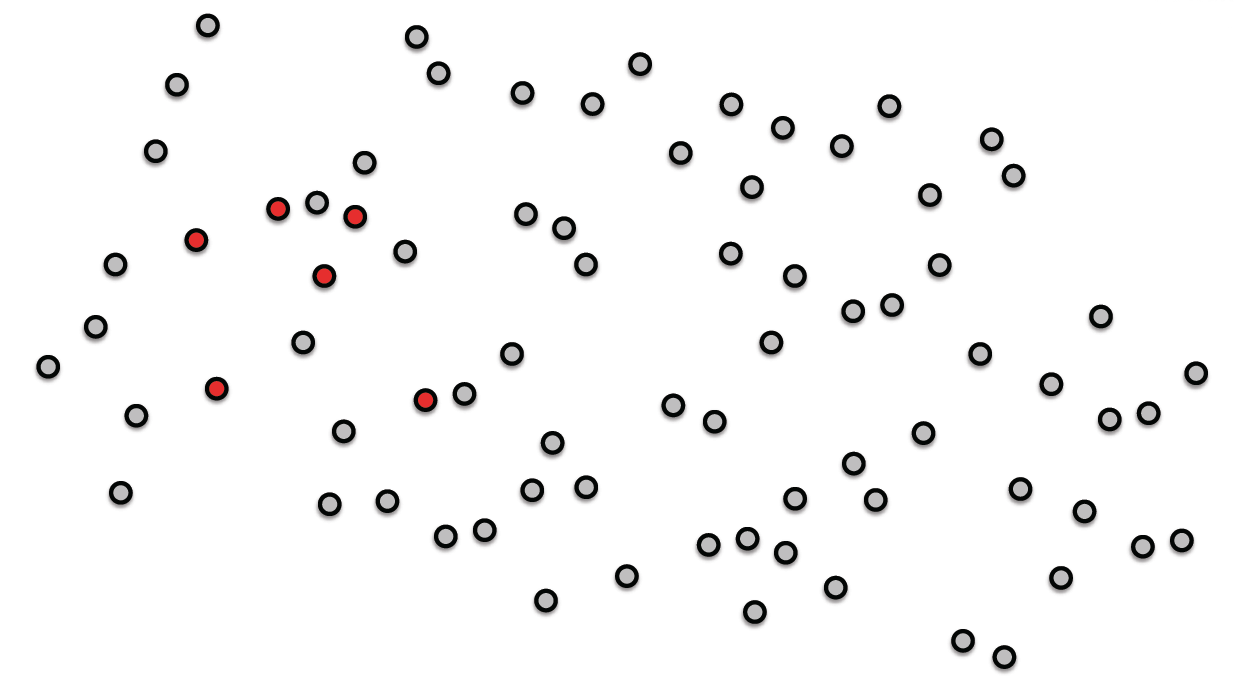
\includegraphics[width=1\textwidth,valign=b]{images/finding_effectors1}    
\end{frame}

% SEQUENCE SPACE
\begin{frame}
  \frametitle{Similarity distance
  \footnote{\tiny{\href{http://dx.doi.org/10.1007/978-1-62703-986-4_4}{Pritchard \& Broadhurst (2014) \textit{Methods Mol. Biol.} doi:10.1007/978-1-62703-986-4\_4}}}
}
  Define a representative \textcolor{hutton_green}{\textit{centre}}, and a \textcolor{hutton_blue}{distance} from it that includes known effectors \vspace{0.5cm}
  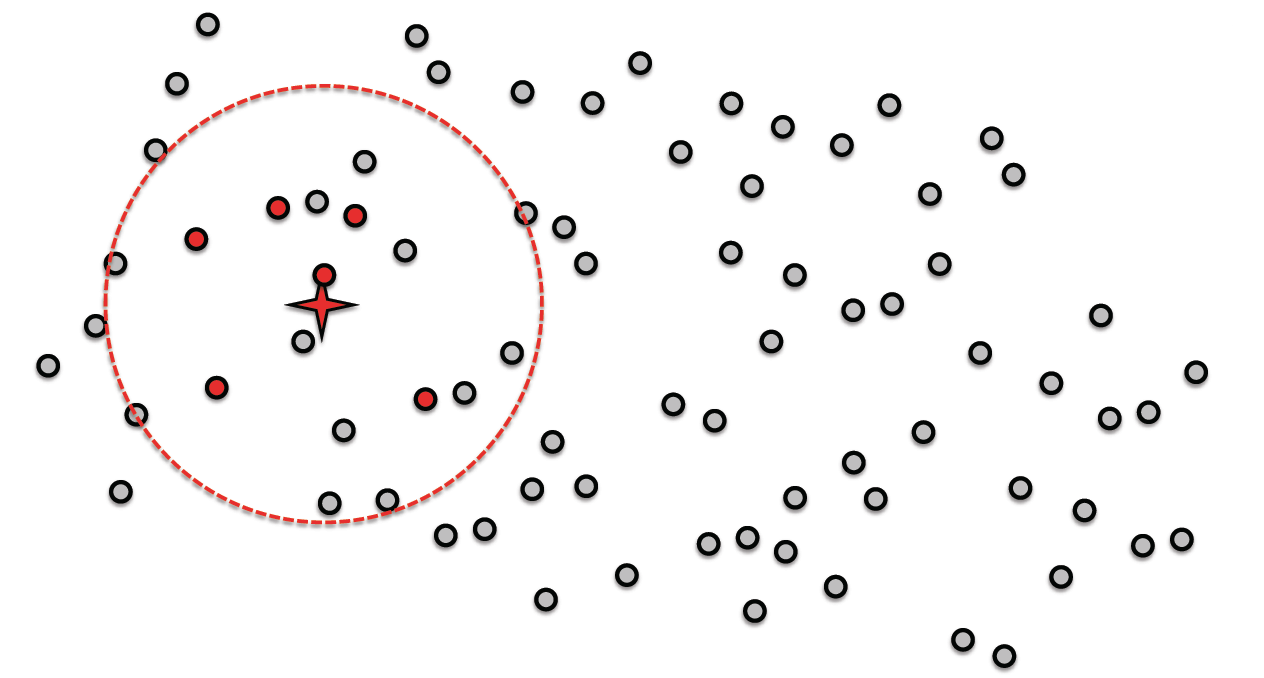
\includegraphics[width=1\textwidth,valign=b]{images/finding_effectors2}    
\end{frame}

% CLASSIFY CANDIDATES
\begin{frame}
  \frametitle{Classify candidates
  \footnote{\tiny{\href{http://dx.doi.org/10.1007/978-1-62703-986-4_4}{Pritchard \& Broadhurst (2014) \textit{Methods Mol. Biol.} doi:10.1007/978-1-62703-986-4\_4}}}
}
  Classify sequences \textcolor{hutton_green}{within the distance} as \textcolor{hutton_blue}{similar} \vspace{0.5cm}
  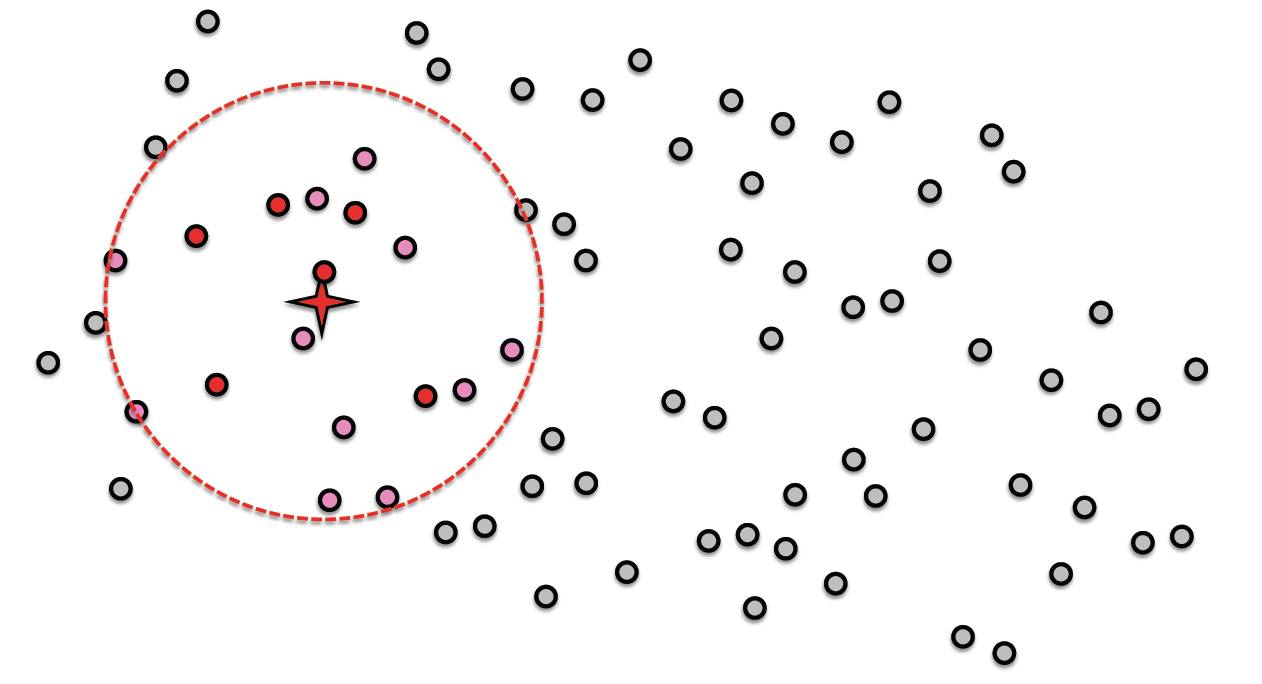
\includegraphics[width=1\textwidth,valign=b]{images/finding_effectors3}    
\end{frame}

% EXERCISE
\begin{frame}
  \frametitle{EXERCISE}
  \begin{alertblock}{\url{exercises/03-effector_finding.ipynb}}
    \begin{itemize}
      \item Downloading annotated \textit{Pseudomonas} AvrPto1 effectors from a public sequence repository
      \item Building a (HMM) model from this training set
      \item Searching public genome annotations with the model
    \end{itemize}
  \end{alertblock}
  \begin{itemize}
    \item \textcolor{hutton_purple}{\href{http://mybinder.org/repo/widdowquinn/Teaching-EMBL-Plant-Path-Genomics}{MyBinder link}}
  \end{itemize}
\end{frame}

% CHOOSING A DISTANCE
\begin{frame}
  \frametitle{Choosing a distance
  \footnote{\tiny{\href{http://dx.doi.org/10.1007/978-1-62703-986-4_4}{Pritchard \& Broadhurst (2014) \textit{Methods Mol. Biol.} doi:10.1007/978-1-62703-986-4\_4}}}
}
  \begin{columns}[T]
    \begin{column}{5cm}  
      \begin{itemize}  
        \item \textcolor{hutton_green}{How do we define distance?}
        \item \textcolor{hutton_blue}{How large a distance should we take?}
        \item \textcolor{hutton_purple}{How do we know if we chose well?}
        \end{itemize}  
      \end{column}
    \begin{column}{5cm}  
      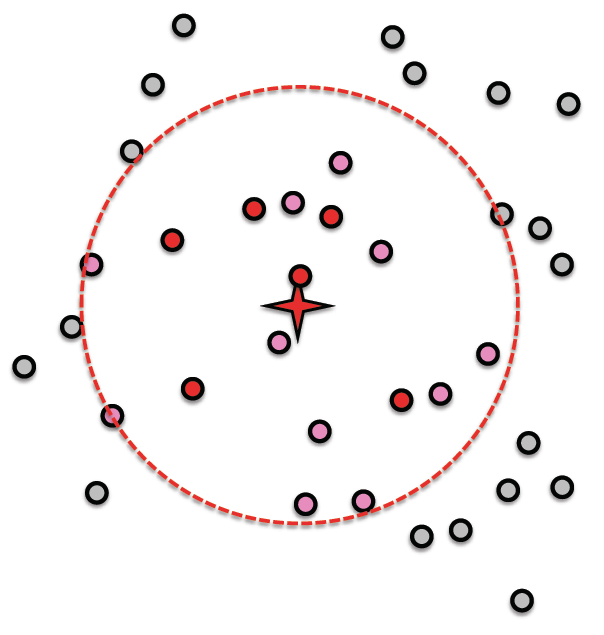
\includegraphics[width=1\textwidth,valign=b]{images/finding_effectors4}    
    \end{column}
  \end{columns}  
\end{frame}

% ARE YOU IN OR OUT? 1
\begin{frame}
  \frametitle{Are you in or out?
  \footnote{\tiny{\href{http://dx.doi.org/10.1007/978-1-62703-986-4_4}{Pritchard \& Broadhurst (2014) \textit{Methods Mol. Biol.} doi:10.1007/978-1-62703-986-4\_4}}}
}
  \begin{itemize}
    \item \textcolor{hutton_green}{The boundary (distance) classifies sequences as `in' or `out'}
    \item Sequences are predicted to be \textit{either} \textcolor{red}{in the class} \textit{or} \textcolor{blue}{not in the class}
    \item \textcolor{hutton_purple}{Changing distance/boundary changes classification}
  \end{itemize}
  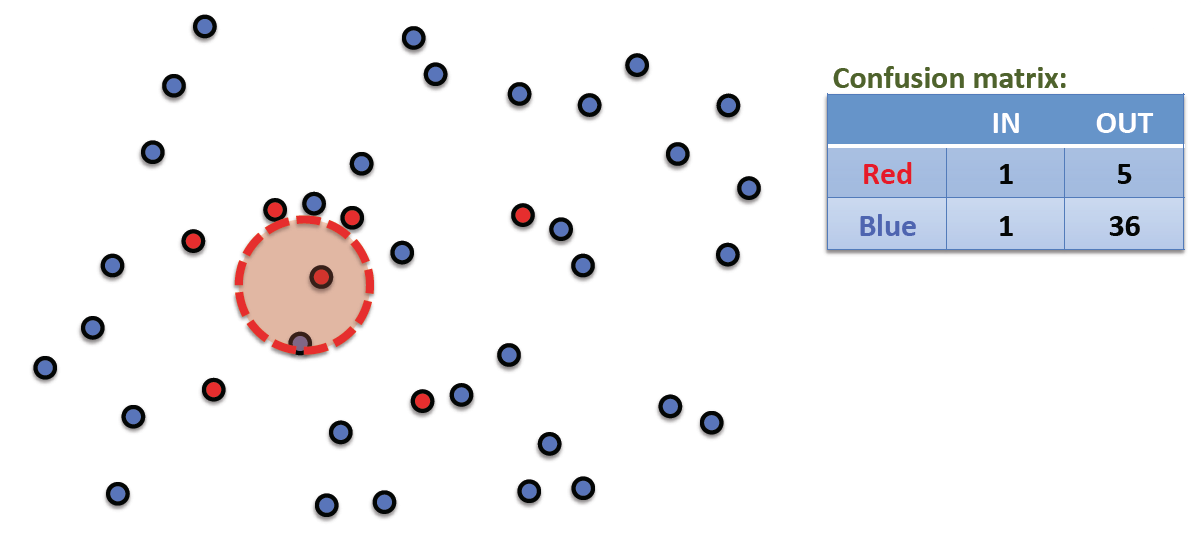
\includegraphics[width=1\textwidth]{images/finding_effectors5}    
\end{frame}

% TP/TN/FP/FN
\begin{frame}
  \frametitle{TP/TN/FP/FN
  \footnote{\tiny{\href{http://dx.doi.org/10.1007/978-1-62703-986-4_4}{Pritchard \& Broadhurst (2014) \textit{Methods Mol. Biol.} doi:10.1007/978-1-62703-986-4\_4}}}
}
  \begin{itemize}
    \item \textcolor{hutton_green}{The boundary (distance) classifies sequences as `in' or `out'}
    \item Sequences are predicted to be \textit{either} \textcolor{red}{in the class} \textit{or} \textcolor{blue}{not in the class}
    \item \textcolor{hutton_purple}{Changing distance/boundary changes classification}
  \end{itemize}
  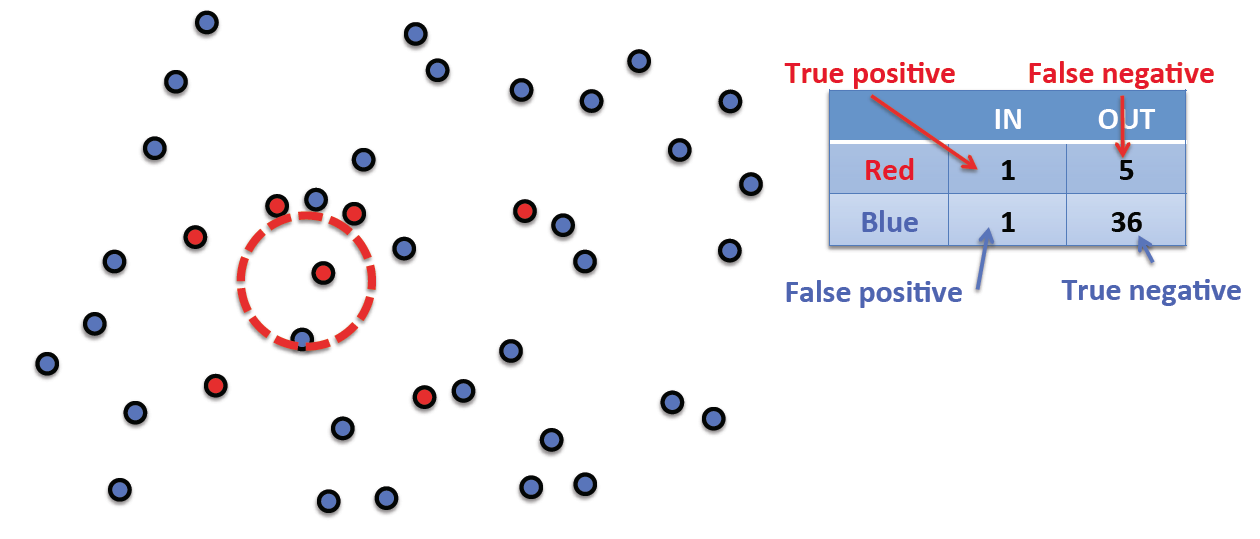
\includegraphics[width=1\textwidth]{images/finding_effectors6}    
\end{frame}

% FPR/FNR/Sn/Sp/FDR
\begin{frame}
  \frametitle{FPR/FNR/Sn/Sp/FDR
  \footnote{\tiny{\href{http://dx.doi.org/10.1007/978-1-62703-986-4_4}{Pritchard \& Broadhurst (2014) \textit{Methods Mol. Biol.} doi:10.1007/978-1-62703-986-4\_4}}}
}
  \begin{itemize}
    \item \textcolor{hutton_green}{The boundary (distance) classifies sequences as `in' or `out'}
    \item Sequences are predicted to be \textit{either} \textcolor{red}{in the class} \textit{or} \textcolor{blue}{not in the class}
    \item \textcolor{hutton_purple}{Changing distance/boundary changes classification}
  \end{itemize}
  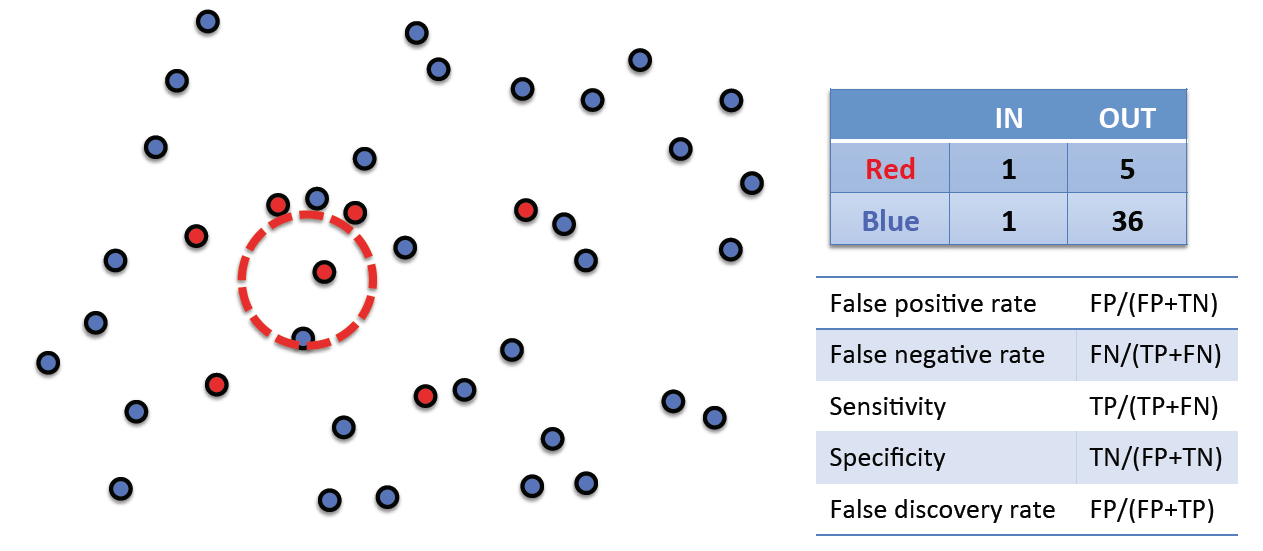
\includegraphics[width=1\textwidth]{images/finding_effectors7}    
\end{frame}

% SMALL BOUNDARY
\begin{frame}
  \frametitle{Small Boundary
  \footnote{\tiny{\href{http://dx.doi.org/10.1007/978-1-62703-986-4_4}{Pritchard \& Broadhurst (2014) \textit{Methods Mol. Biol.} doi:10.1007/978-1-62703-986-4\_4}}}
}
  \begin{itemize}
    \item \textcolor{hutton_green}{The boundary (distance) classifies sequences as `in' or `out'}
    \item Sequences are predicted to be \textit{either} \textcolor{red}{in the class} \textit{or} \textcolor{blue}{not in the class}
    \item \textcolor{hutton_purple}{Changing distance/boundary changes classification}
  \end{itemize}
  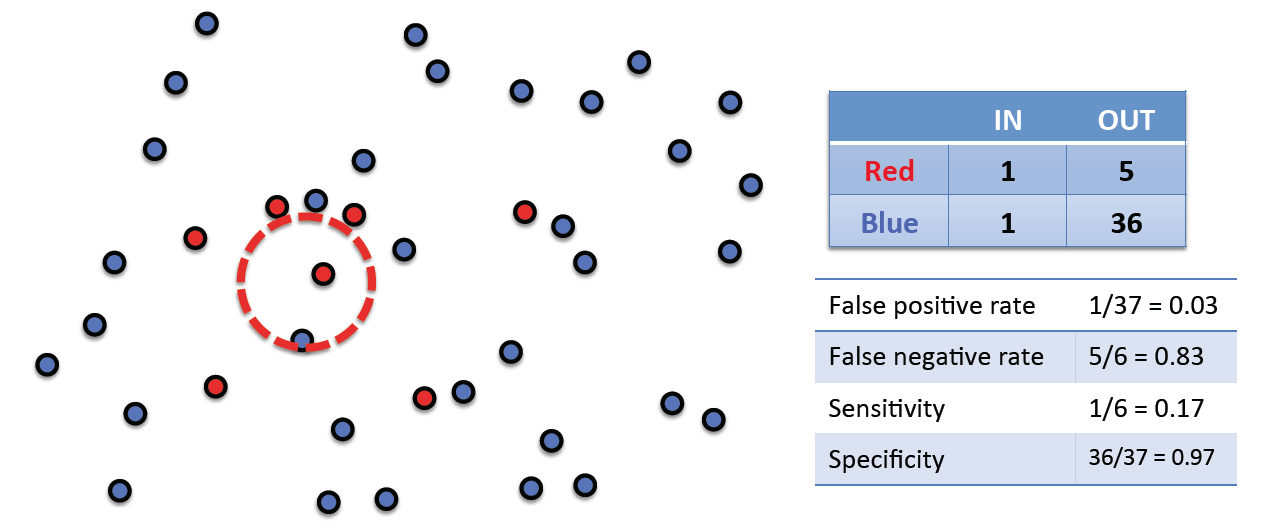
\includegraphics[width=1\textwidth]{images/finding_effectors8}    
\end{frame}

% MEDIUM BOUNDARY
\begin{frame}
  \frametitle{Medium boundary
  \footnote{\tiny{\href{http://dx.doi.org/10.1007/978-1-62703-986-4_4}{Pritchard \& Broadhurst (2014) \textit{Methods Mol. Biol.} doi:10.1007/978-1-62703-986-4\_4}}}
}
  \begin{itemize}
    \item \textcolor{hutton_green}{The boundary (distance) classifies sequences as `in' or `out'}
    \item Sequences are predicted to be \textit{either} \textcolor{red}{in the class} \textit{or} \textcolor{blue}{not in the class}
    \item \textcolor{hutton_purple}{Changing distance/boundary changes classification}
  \end{itemize}
  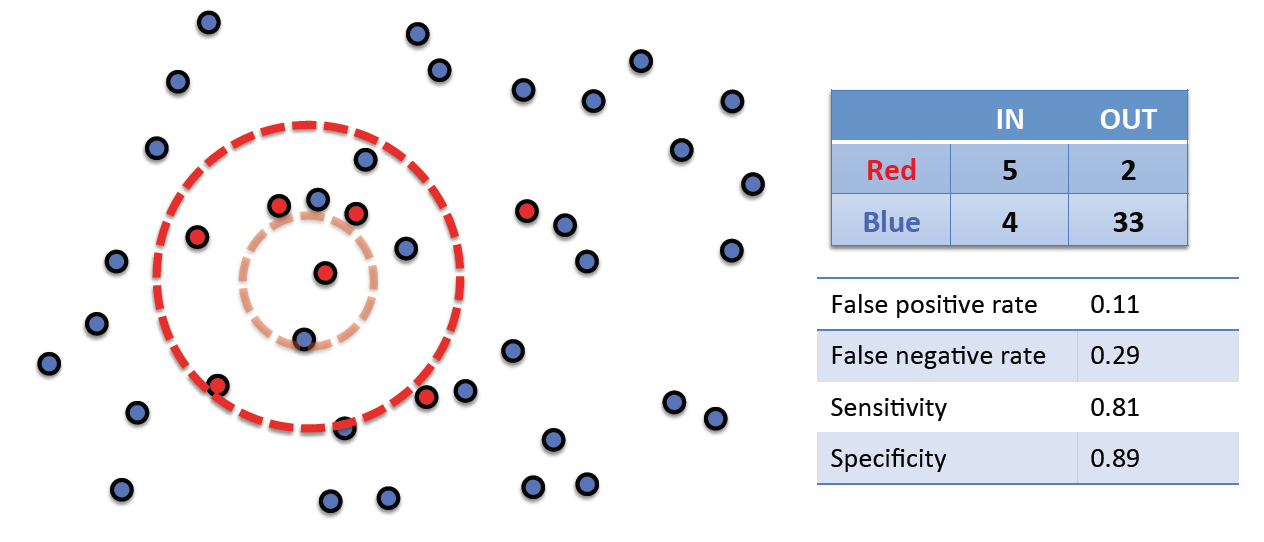
\includegraphics[width=1\textwidth]{images/finding_effectors9}    
\end{frame}

% LARGE BOUNDARY
\begin{frame}
  \frametitle{Large boundary
  \footnote{\tiny{\href{http://dx.doi.org/10.1007/978-1-62703-986-4_4}{Pritchard \& Broadhurst (2014) \textit{Methods Mol. Biol.} doi:10.1007/978-1-62703-986-4\_4}}}
}
  \begin{itemize}
    \item \textcolor{hutton_green}{The boundary (distance) classifies sequences as `in' or `out'}
    \item Sequences are predicted to be \textit{either} \textcolor{red}{in the class} \textit{or} \textcolor{blue}{not in the class}
    \item \textcolor{hutton_purple}{Changing distance/boundary changes classification}
  \end{itemize}
  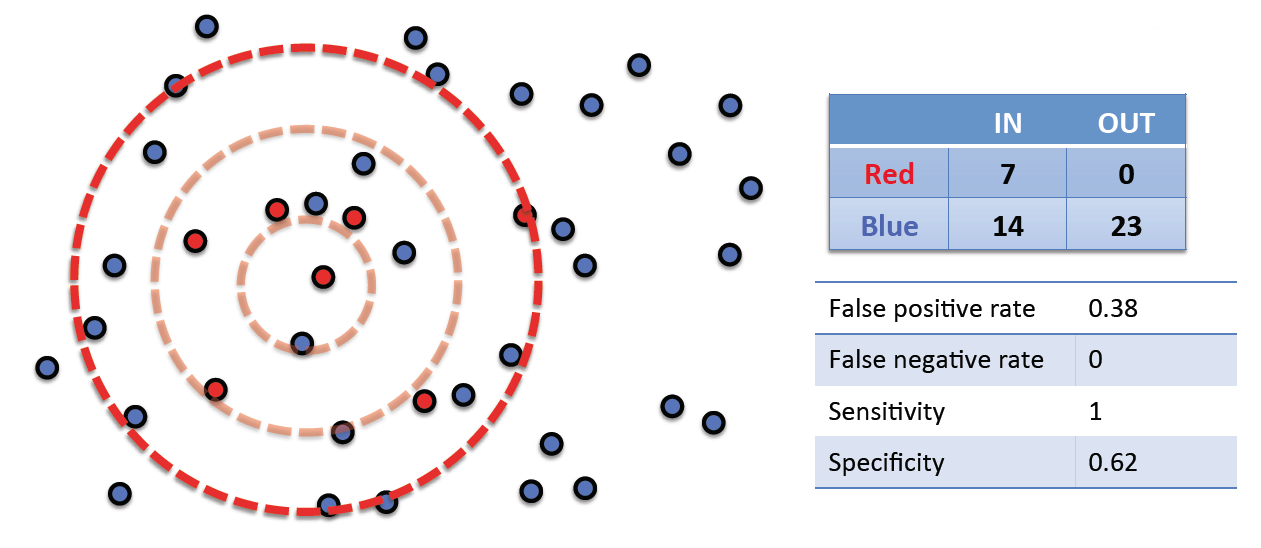
\includegraphics[width=1\textwidth]{images/finding_effectors10}    
\end{frame}

% CHOOSING A BOUNDARY
\begin{frame}
  \frametitle{Choosing a boundary
  \footnote{\tiny{\href{http://dx.doi.org/10.1007/978-1-62703-986-4_4}{Pritchard \& Broadhurst (2014) \textit{Methods Mol. Biol.} doi:10.1007/978-1-62703-986-4\_4}}}
}
  \begin{columns}[T]
    \begin{column}{5cm}  
      \begin{itemize}  
        \item \textcolor{hutton_green}{Assign known `positive` and `negative' examples}
        \item \textcolor{hutton_blue}{Vary `distance' and measure predictive performance (F-measure, AUC, $\ldots$}
        \item \textcolor{hutton_purple}{Choose the distance that gives the `best' performance}
        \end{itemize}  
      \end{column}
    \begin{column}{5cm}  
      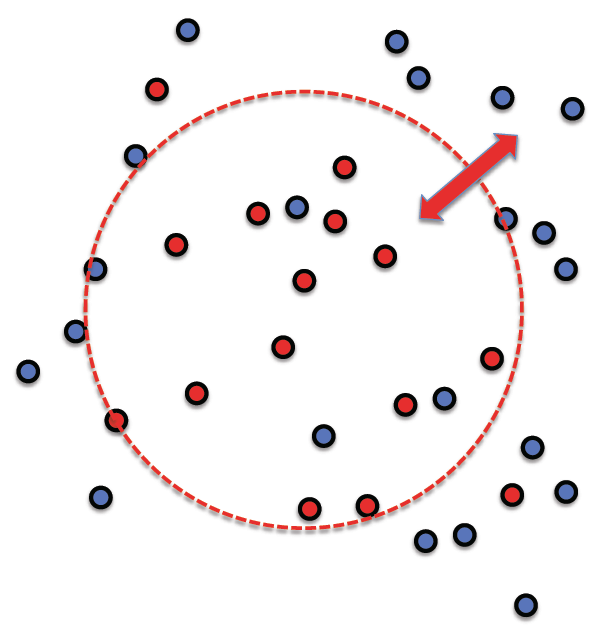
\includegraphics[width=1\textwidth]{images/finding_effectors11}    
    \end{column}
  \end{columns} 
\end{frame}

% CROSSVALIDATION
\begin{frame}
  \frametitle{Crossvalidation
    \footnote{\tiny{\href{http://dx.doi.org/10.1007/978-1-62703-986-4_4}{Pritchard \& Broadhurst (2014) \textit{Methods Mol. Biol.} doi:10.1007/978-1-62703-986-4\_4}}}
}
      \begin{itemize}  
        \item \textcolor{hutton_green}{Estimation of classifier performance depends on:}
          \begin{itemize}
            \item Boundary choice/distance measure
            \item Composition of training set (`positives' and `negatives')
          \end{itemize}
        \item \textcolor{hutton_blue}{Cross-validation gives objective estimate of performance}
        \item \textcolor{hutton_purple}{Many strategies (beyond today's scope), including:}
          \begin{itemize}
            \item leave-one-out (LOO)
            \item $k$-fold crossvalidation
            \item repeated (random) subsampling
          \end{itemize}
        \item \textcolor{red}{Always validate against a \textit{hold-out set} (not used to train the classifier)}
        \end{itemize}          
\end{frame}

% POST-CROSSVALIDATION
\begin{frame}
  \frametitle{Post-crossvalidation
  \footnote{\tiny{\href{http://dx.doi.org/10.1007/978-1-62703-986-4_4}{Pritchard \& Broadhurst (2014) \textit{Methods Mol. Biol.} doi:10.1007/978-1-62703-986-4\_4}}}
}
  \begin{itemize}
    \item \textcolor{hutton_green}{Crossvalidation gives `best' method \& parameters}
    \item \textcolor{hutton_purple}{Apply `best' method to complete dataset for prediction}
  \end{itemize}
  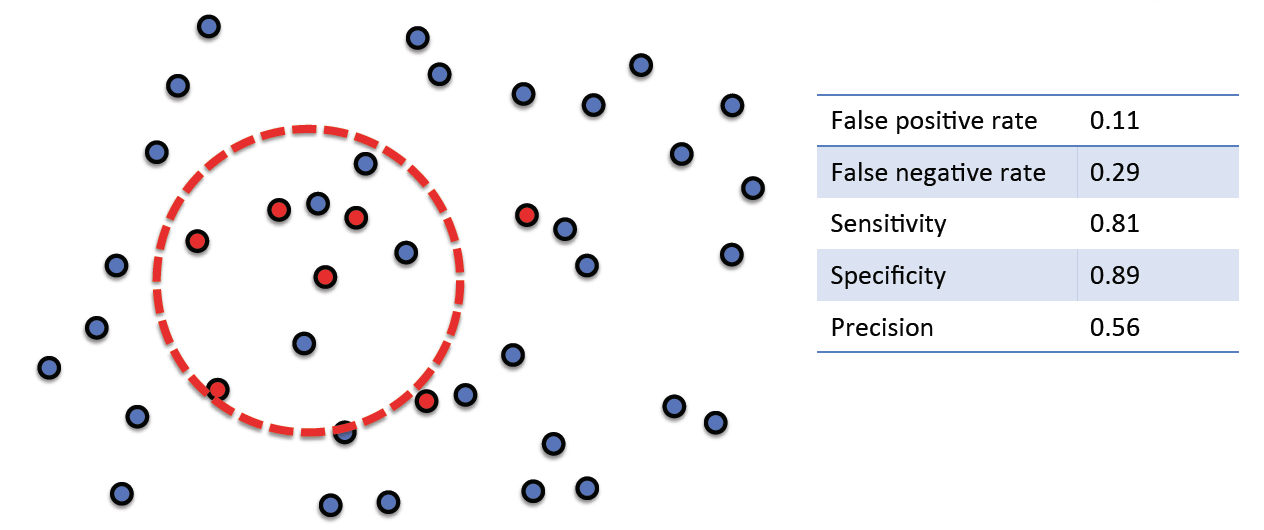
\includegraphics[width=1\textwidth]{images/finding_effectors12}    \\
  \textcolor{red}{BEWARE THE BASERATE FALLACY!}
\end{frame}

% OPTIONAL WORKSHEET
\begin{frame}
  \frametitle{OPTIONAL WORKSHEET}
  \begin{alertblock}{\url{worksheets/03-effector-finding.ipynb}}
    The Baserate Fallacy in effector prediction and classification.
  \end{alertblock}
  \begin{itemize}
    \item \textcolor{hutton_purple}{\href{http://mybinder.org/repo/widdowquinn/Teaching-EMBL-Plant-Path-Genomics}{MyBinder link}}
  \end{itemize}
\end{frame}